\documentclass[a4paper, 10pt]{article}
\usepackage{header}

\title{\LARGE{Теория вероятностей и математическая статистика—2}}
\author{Винер Даниил  \href{https://t.me/danya_vin}{@danya\_vin}}
\date{Версия от \today}
\begin{document}
\maketitle
\tableofcontents
\setlength{\parindent}{15pt}
\setlength{\parskip}{2mm}
\setlist[itemize]{left=1cm}
\setlist[enumerate]{left=1cm}
\newpage
\section{Закон больших чисел. Центральная предельная теорема}
\subsection{Закон больших чисел в форме Бернулли}
Пусть имеются некоторые случайные величины $\xi_i=\begin{cases}
    1,&p\\
    0,&1-p
\end{cases}$, где $p$ — вероятность, что какое-то событие произошло. Тогда $\matwait{\xi}=p$, $\dispersia{\xi}=p(1-p)\leqslant \frac{1}{4}$

\theorem Пусть $\hat{p}=\frac{1}{n}\sum_{i=1}^{n} \xi_i$ — доля успехов в $n$ испытаниях Бернулли, тогда $\hat{p}\overset{p}{\longrightarrow} p$

\proof Распишем по неравенству Чебышёва: 
\begin{equation*}
    \prob{|\hat{p}-p|\geqslant\ve}\leqslant\frac{p(1-p)}{n\ve^2}\leqslant \frac{1}{4n\ve^2}\underset{n\to\infty}{\longrightarrow}0
\end{equation*}

\subsection*{Пример}
Пусть 87\% новорожденных доживают до 50 лет. Тогда $p=0,87$ — вероятность дожить до 50. Рассмотрим $n=1000$ новорожденных

Опредедлим с какой вероятностью данная случайная величина отклонится от своего математического ожидания не более, чем на $0,04$ — $\prob{|\hat{p}-0,87|\leqslant 0,04}$. По Чебышёву:
\begin{equation*}
    \prob{|\hat{p}-p|\leqslant 0,04}\geqslant1-\frac{\dispersia{\hat{p}}}{(0,04)^2}=1-\frac{0,87\cdot0,13}{0,0016\cdot1000}=0,929
\end{equation*}

\subsection{Центральная предельная теорема}
Рассмотрим сумму независимых одинаково распределенных случайных величин:
\begin{equation*}
    S_n=\xi_1+\ldots+\xi_n,
\end{equation*}
при этом существует $\dispersia{\xi_i}\leqslant c$, $\matwait{\xi_i}=\mu$, $\dispersia{\xi_n}=\sigma^2$

Тогда, $Z_n=\displaystyle\frac{S_n-n\mu}{\sqrt{n\sigma^2}}\overset{d}{\longrightarrow}Z$, где $Z\sim \mathcal{N}(0;1)$ — имеет стандартное нормальное распределение

Функция плотности:
\begin{equation*}
    \varphi(z)=\frac{1}{\sqrt{2\pi}}e^{\frac{-z^2}{2}}
\end{equation*}


\subsection{Теорема Муавра-Лапласа}
\theorem Имеется $\xi_i=\begin{cases}
    1,&p\\
    0,&1-p
\end{cases}$. $S_n=\sum \xi_i$ — число успехов в $n$ испытаниях. Тогда
\begin{equation*}
    Z_n=\frac{S_n-np}{\sqrt{np(1-p)}}\overset{d}{\longrightarrow}Z\sim \mathcal{N}(0;1)
\end{equation*}



\subsection*{Пример}
Проходит суд над Бенджамином Споком. Из 300 человек 90 — женщины, которые симпатизируют Споку, при этом 12 присяжных будут судить Спока. Требуется определить мог ли отбор присяжных быть случайным.

Число успехов в данном случае — число женщин среди 300 присяжных. Будем считать, что $p=0.5$, то есть половина женщин.

\begin{equation*}
    \prob{\frac{S_{300}-150}{\sqrt{0.5\cdot0.5\cdot300}}\leqslant \frac{90-150}{\sqrt{75}}}\simeq\Phi(-6.93)\simeq2.3\cdot10^{-12}
\end{equation*}

Значит, практически невозможно случайным образом выбрать 90 или меньше женщин среди 300 присяжных при справедливом распределении, то есть отбор был предвзятым


\subsection{Неравенство Берри-Эссена}
\begin{equation*}
    |F_n-\Phi|\leqslant\frac{C_0\cdot\matwait{|\xi_1-\mu|^3}}{\sigma^3\sqrt{n}},\text{ где }\begin{cases}
        F_n\text{ — функция распределения стандартизированной СВ}\\
        C_0\text{ — константа}\\
        \matwait{|\xi_1-\mu|^3}\text{ — третий абсолютный центральный момент}
    \end{cases}
\end{equation*}



\subsection*{Пример}
Пусть имеется $n=1000$ заключенных договоров страхования с 1 января на 1 год. С вероятностью $p=0.05$ произойдет страховой случай, выплаты по каждому договору — 2000 у.е. $R$ — резерв страховой компании

Требуется определить какой должен быть размер резерва, чтобы страховая компания выполнила свои обязательства с вероятностью $0.99$

$S_n=2000(\xi_1+\ldots+\xi_n)$, $\xi_i\sim Bi(p=0.05)$

\begin{equation*}
    \prob{S_n\leqslant R}=\prob{\frac{\sum\xi_i-0.05\cdot1000}{\sqrt{1000\cdot0.05\cdot0.95}}\leqslant \frac{\frac{R}{2000}-0.05\cdot1000}{\sqrt{1000\cdot0.05\cdot0.95}}}\geqslant 0,99
\end{equation*}
Значит, требуется найти квантиль уровня $0.99$. Он равен $2.33$, тогда
\begin{equation*}
    \frac{\frac{R}{2000}-0.05\cdot1000}{\sqrt{1000\cdot0.05\cdot0.95}}=2.33\Longrightarrow R=132117
\end{equation*}
То есть, для покрытия 99\% страховых случаев у страховой компании резерв должен быть размером $132117$ у.е. Напротив, для покрытия всех случаев $R=2000000$




\newpage
\section{Многомерное нормальное распределение}
\subsection{Одномерное нормальное распределение}
\definition Случайная величина имеет нормальное распределение $X\sim\mathcal{N}(\mu,\sigma^2)$, если функция плотности равна
\begin{equation*}
    f_X(x)=\frac{1}{\sqrt{2\pi}\sigma}e^{-\frac{1}{2}\left(\frac{x-\mu}{\sigma}\right)^2}
\end{equation*}


\subsection{Многомерное нормальное распределение—1}
\definition Пусть случайные величины $z_1,\ldots,z_n$ независимы и $\sim N(0,1)$. Тогда $z=\begin{pmatrix}
    z_1\\
    \vdots\\
    z_n
\end{pmatrix}$ имеет многомерное нормальное распределение $N(0,I)$, где $I$ — единичная матрица

Функция плотности:
\begin{equation*}
    f_Z(z)=\frac{1}{(\sqrt{2\pi})^n}e^{-\frac{1}{2}\sum_{i=1}^n z_i^2}=\frac{1}{(\sqrt{2\pi})^n}e^{-0.5Z^TZ}
\end{equation*}


\comment Пусть $Z\sim N(0,I)$, $A\in\text{Mat}_{k\times n}$ — матрица полного ранга и $k<n$, то есть rank$A=k$. Тогда
\begin{equation*}
    Y=AZ+b\sim N(b,AA^T)
\end{equation*}
\begin{equation*}
    \begin{aligned}
        f_Y(y)&=\frac{1}{|\det A|}f_Z(A^{-1}(y-b))\\
        &=\frac{1}{(\sqrt{2\pi})^n}\frac{1}{|\det A|}e^{-0.5(y-b)^T(A^{-1})^TA^{-1}(y-b)}\\
        &\text{пусть }AA^T=C\\
        &=\frac{1}{(\sqrt{2\pi})^n}\frac{1}{\sqrt{|C|}}e^{-0.5(y-b)^TC^{-1}(y-b)}
    \end{aligned}
\end{equation*}


\begin{definition}
    Случайная величина $Y\sim N(b,C)$, если
    \begin{equation*}
        f_Y(y)=\frac{1}{(\sqrt{2\pi})^n}\frac{1}{\sqrt{|C|}}e^{-0.5(y-b)^TC^{-1}(y-b)}
    \end{equation*}
\end{definition}

\begin{definition}
    Случайный вектор $Y\sim N(0,C)$, если $\forall a_1,\ldots,a_n$
    \begin{equation*}
        a_1Y_1+a_2Y_2+\ldots+a_nY_n
    \end{equation*}
    либо $N(0,\dot)$ либо const
\end{definition}


\subsection{Свойства многомерного нормального распределения}
Пусть $Y\sim N(b,C)$
\begin{enumerate}
    \item $\matwait{Y}=b,cov(Y)=C$
    
    \proof $Y=AZ+b$, $Z\sim N(0,I)$
    \begin{equation*}
        \begin{aligned}
            cov(Y)=\matwait{(AZ+b-\matwait{AZ+b})(AZ+b-AEZ-b)^T}=AcovZA^T=AA^T=C
        \end{aligned}
    \end{equation*}
    \item Любое линейное невырожденное преобразование многомерного нормаьного дает многомерный нормальный вектор
    
    $\forall B,a:$ $BY+a\sim N(Bb+a,BCB^T)$

    \item $\forall$ подвектор нормального вектора нормален 
    \item Если $Y\sim N(b,D)$, то его компоненты независимы
    
    \comment Некоррелированность = независимость

    \proof 
    \begin{equation*}
        \begin{aligned}
            f_Y(y)&=\frac{1}{(\sqrt{2\pi}^n)}e^{-0.5(y-b)^T D^{-1}(y-b)}\\
            &=\frac{1}{(\sqrt{2\pi}^n)}e^{-0.5\sum \left(\frac{y_i-b_i}{\sigma_i}\right)^2}\\
            &=\prod_{i=1}^n\frac{1}{\sqrt{2\pi}}e^{-0.5\left(\frac{y_i-b_i}{\sigma_i}\right)^2}
        \end{aligned}
    \end{equation*}
\end{enumerate}

\ex $Y_1\sim N(0,1),\ \lambda=\begin{cases}
    1,&p=0.5\\
    -1,&p=0.5
\end{cases},\ Y_2=2Y_1$

\begin{equation*}
    \begin{aligned}
        \prob{Y_2\leqslant y}&=\prob{Y_1\leqslant y|\alpha=1}\cdot\prob{\alpha=1}+\prob{-Y_1\leqslant y|\alpha=-1}\cdot\frac{1}{2}\\
        &=\Phi(y)
    \end{aligned}
\end{equation*}

$cov(Y_1,Y_2)=cov(Y_1,2Y_1)=\matwait{\alpha Y_1^2}-\matwait{Y}\matwait{\alpha Y_1}=0$. То есть они не коррелированы


\subsection{Условное нормальное распределение}
Имеется случайный вектор $\begin{pmatrix}
    z_1\\
    z_2
\end{pmatrix}\sim N\left(\begin{pmatrix}
    0\\
    0
\end{pmatrix},\begin{pmatrix}
    1&\rho\\
    \rho&1
\end{pmatrix}\right)$, пишут $\Phi_2(z_1,z_2;\rho)$

Допустим, что $z_1$ фиксирован, тогда $z_2|z_1=z\sim N(\rho z,1-\rho^2)$

$z_2=\rho z_1+u$, где $z_1$ и $u$ независимы и $u\sim N(.,.)$

\newpage
\section{Многомерное нормальное распределение—2}
\subsection{Условное нормальное распределение}
%\begin{enumerate}
    %\item 
    $\begin{pmatrix}
        z_1\\
        z_2
    \end{pmatrix}\sim N\left(\begin{pmatrix}
        0\\
        0
    \end{pmatrix},\begin{pmatrix}
        1&\rho\\
        \rho&1
    \end{pmatrix}\right)$, пишут $\Phi_2(z_1,z_2;\rho)$
    
    Допустим, что $z_1$ фиксирован, тогда $z_2|z_1=z\sim N(\rho z,1-\rho^2)$

    \state $z_2=\rho z_1+u$, где $z_1$ и $u$ независимы и $(u,z_1)\sim N(.,.)$

    \proof $u=z_1-\rho z_1\Longrightarrow (z_1, u)=(z_1, z_2-\rho z_1)=\begin{pmatrix}
        1&0\\
        -\rho & 1
    \end{pmatrix}\begin{pmatrix}
        z_1\\
        z_2
    \end{pmatrix}\sim N\left(\begin{pmatrix}
        0\\
        0
    \end{pmatrix},\begin{pmatrix}
        1&0\\
        0&1-\rho^2
    \end{pmatrix}\right)$

    $cov(z_1, u)=A\cdot cov(z_1,z_2)\cdot A^T=\begin{pmatrix}
        1&0\\
        0&1-\rho^2
    \end{pmatrix}$\qed

    \textbf{Доказательство свойства.} $\matwait{z_2}=\rho\matwait{z_1}+\matwait{u}=0$, $\dispersia{z_2}=\rho^2\dispersia{z_1}+\dispersia{u}=\rho^2+1-\rho^2=1$

    $(z_2\vert z_1=z)=\rho z+u\Longrightarrow \begin{cases}
        \matwait{z_2\vert z_1=z}=\rho z+\matwait{u}=\rho z\\
        \dispersia{z_2\vert z_1=z}=\dispersia{u}=1-\rho^2
    \end{cases}$\qed

    \comment Пусть вектор $Y$ такой, что $AY\sim N(.,.)$ (многомерное нормальное), меньшей размерности, чем $Y$, тогда говорят, что $Y$ имеет обобщенное нормальное распределение


%\end{enumerate}

\comment Двумерная Гауссова копула представима в виде $\Phi_2(\Phi^{-1}(F_1(u_1)),\Phi^{-1}(F_2(u_2));\rho)$


\subsection{Многомерная центральная предельная теорема}
\theorem Пусть $\xi^{(1)}_1,\ldots,\xi^{(n)}_n$ — последовательность независимых одинаково распределенных случайных векторов, у каждого из которых $\matwait{\xi^{(k)}}=b\ \forall k$, $cov(\xi^{(k)})=c,\ \det C>0$. 

Обозначим $S_n=\xi^{(1)}_1+\ldots+\xi^{(n)}_n$ — вектор частичных сумм. Тогда, при $n\to\infty$ последовательность $\eta^{(n)}$, где $\eta^{(n)}=\frac{S_n-nb}{\sqrt{n}}$ сходится по распределению к вектору $\eta\sim N\left(\overrightarrow{0},C\right)$

% Для одномерного: $S_n=\xi_1+\ldots+\xi_n$, $\frac{S_n-n\mu}{\sqrt{n\sigma^2}}\sim N(0,\sigma^2)$

\newpage
\section{TBA}

\newpage
\section{Введение в математическую статистику}
\begin{itemize}
    \item Имеется $n$ независимых случайных величин $X_1,\ldots,X_n$, которые имеют одинаковые функции распределения: $F_{X_1}(x)=\ldots=F_{X_n}(x)=F(x)$
    \item Пусть функция распределения $F(x)$ зависит от некоторого вектора неизвестных параметров $\theta=(\theta_1,\ldots,\theta_r)$
    \item $F(x)=F(x;\theta)$, где $x$ — переменная, а $\theta$ — вектор неизвестных параметров
    \item $\Theta$ — множество допустимых значений вектора $\theta$
    
    \ex Если $X_i\sim N(\mu,\sigma^2)$, то $\theta=(\mu,\sigma^2)\in(-\infty,+\infty)\times(0;+\infty)$
\end{itemize}

\definition Случайной выборкой объема $n$ наблюдений из распределения с функицей распределения $F(x;\theta)$ называется случайный вектор $X=(X_1,\ldots,X_n)$, компоненты которого удовлетворяют следующим условиям
\begin{itemize}
    \item случайные величины $X_1,\ldots,X_n$ — независимы 
    \item случайные величины $X_1,\ldots,X_n$ имеют одну и ту же функцию распределения $F(x;\theta)$:
    \begin{equation*}
        F_{X_1}(x;\theta)=\ldots=F_{X_n}(x;\theta)=F(x;\theta)
    \end{equation*}
\end{itemize}

\comment Продифференцировав эти равенства, получаем, что все функции плотностей распределения равны

\comment Если все величины $X_1,\ldots,X_n$ дискретны, то они должны иметь одинаковые таблицы распределения

\comment При $i\ne j:\ cov(X_i,X_j)=\matwait{X_iX_j}-\matwait{X_i}\cdot\matwait{X_j}=0$, так как $X_i$ и $X_j$ независимы

Имеются случайные величины $X_1(\omega),\ldots,X_n(\omega)$. Пусть произошел вероятностый эксперимент, в результате которого реализовался исход $\omega_0\in\Omega$. То есть 
\begin{equation*}
    X_1(\omega_0),\ldots,X_n(\omega_0)
\end{equation*}
Тогда, вектор $x=(X_1(\omega_0),\ldots,X_n(\omega_0))$ называется \textit{реализацией случайной выборки}

\ex $\Omega=\{a,b,c,d,e,f,g,h\},\ \fk =$ все подмножества $\Omega$

% \begin{equation*}
    \begin{tabular}{c|c|c|c|c|c|c|c|c}
        $\omega$ & a & b& c &d &e &f &g &h\\
        \hline
        $\prob{\omega}$ & $p^3$ & $p^2q$ & $p^2q$ & $pq^2$ & $p^2q$ & $pq^2$ & $pq^2$ & $q^3$\\
        \hline 
        $X_1(\omega)$ & 1 &1& 1& 1& 0& 0& 0& 0\\
        \hline
        $X_2(\omega) $& 1 &1& 0& 0& 1& 1& 0& 0\\
        \hline
        $X_3(\omega)$ &1& 0& 1& 0& 1 &0 &1 &0
    \end{tabular}
% \end{equation*}
\begin{itemize}
    \item $\prob{X_1=1}=p^3+p^2q+p^2q+pq^2=p(p^2+pq+pq+q^2)=p\Longrightarrow X_1\sim Be(p)$

    \item $\prob{X_2=1}=p^3+p^2q+p^2q+pq^2=p(p^2+pq+pq+q^2)=p\Longrightarrow X_2\sim Be(p)$
    
    \item $\prob{X_3=1}=p^3+p^2q+p^2q+pq^2=p(p^2+pq+pq+q^2)=p\Longrightarrow X_3\sim Be(p)$
\end{itemize}

\begin{equation*}
    \begin{aligned}
        \mathbb{P}(\{X_1=1\}\cap\{X_2=1\}\cap\{X_3=1\})&=p^3\\
        \prob{X_1=1}\cdot\prob{X_2=1}\cdot\prob{X_3=1}&=p^3
    \end{aligned}
\end{equation*}
Рассуждая аналогично, перебираем оставшиеся 7 случаев и получаем, что $X_1,X_2,X_3$ — независимы

Пусть $\omega_0=c$, тогда $\left(X_1(\omega_0),X_2(\omega_0),X_3(\omega_0)\right)=(1,0,1)$

\begin{itemize}
    \item Пусть $X=(X_1,\ldots,X_n)$ — случайная выборка
    \item Для каждого $\omega\in\Omega$ расположим числа $X_1(\omega),\ldots,X_n(\omega)$ в порядке возрастания
    \item Получим набор чисел $X_{(1)}(\omega)\leqslant\ldots\leqslant X_{(n)}(\omega)$, где $(i)$ означает уже отсортированный номер
    
    При этом $X_{(1)}(\omega)=\min(X_1(\omega),\ldots,X_n(\omega))$, а $X_{(n)}(\omega)=\max(X_1(\omega),\ldots,X_n(\omega))$
\end{itemize}

\definition Набор случайных величин $X_{(1)},\ldots,X_{(n)}$ называется вариационным рядом

\definition $\overline{X}:=\displaystyle\frac{X_1+\ldots+X_n}{n}$ — выборочное среднее

\definition $s^2:=\displaystyle\frac{1}{n}\sum_{i=1}^n (X_i-\overline{X})^2$ — выборочная дисперсия

\definition $\hat{\sigma^2}:=\displaystyle\frac{1}{n-1}\sum_{i=1}^n (X_i-\overline{X})^2$ — исправленная выброчная дисперсия

\definition \begin{equation*}
    \begin{aligned}
        \hat{F_n}(x)&=\displaystyle\frac{\text{число элементов случайной выборки, которые нестрого меньше } x}{n}\\
        &=\frac{\#\{i\in\{1,\ldots,n\}:\ X_i\leqslant x\}}{n}
        % &=\frac{1}{n}\sum_{i=1}^n 
    \end{aligned}
\end{equation*}

\ex Рассмотрим $\hat{F_3}(x;\omega=c)$ и выборку $(1,0,1)$. Тогда график будет выглядеть так

\begin{figure}[h]
    \centering
    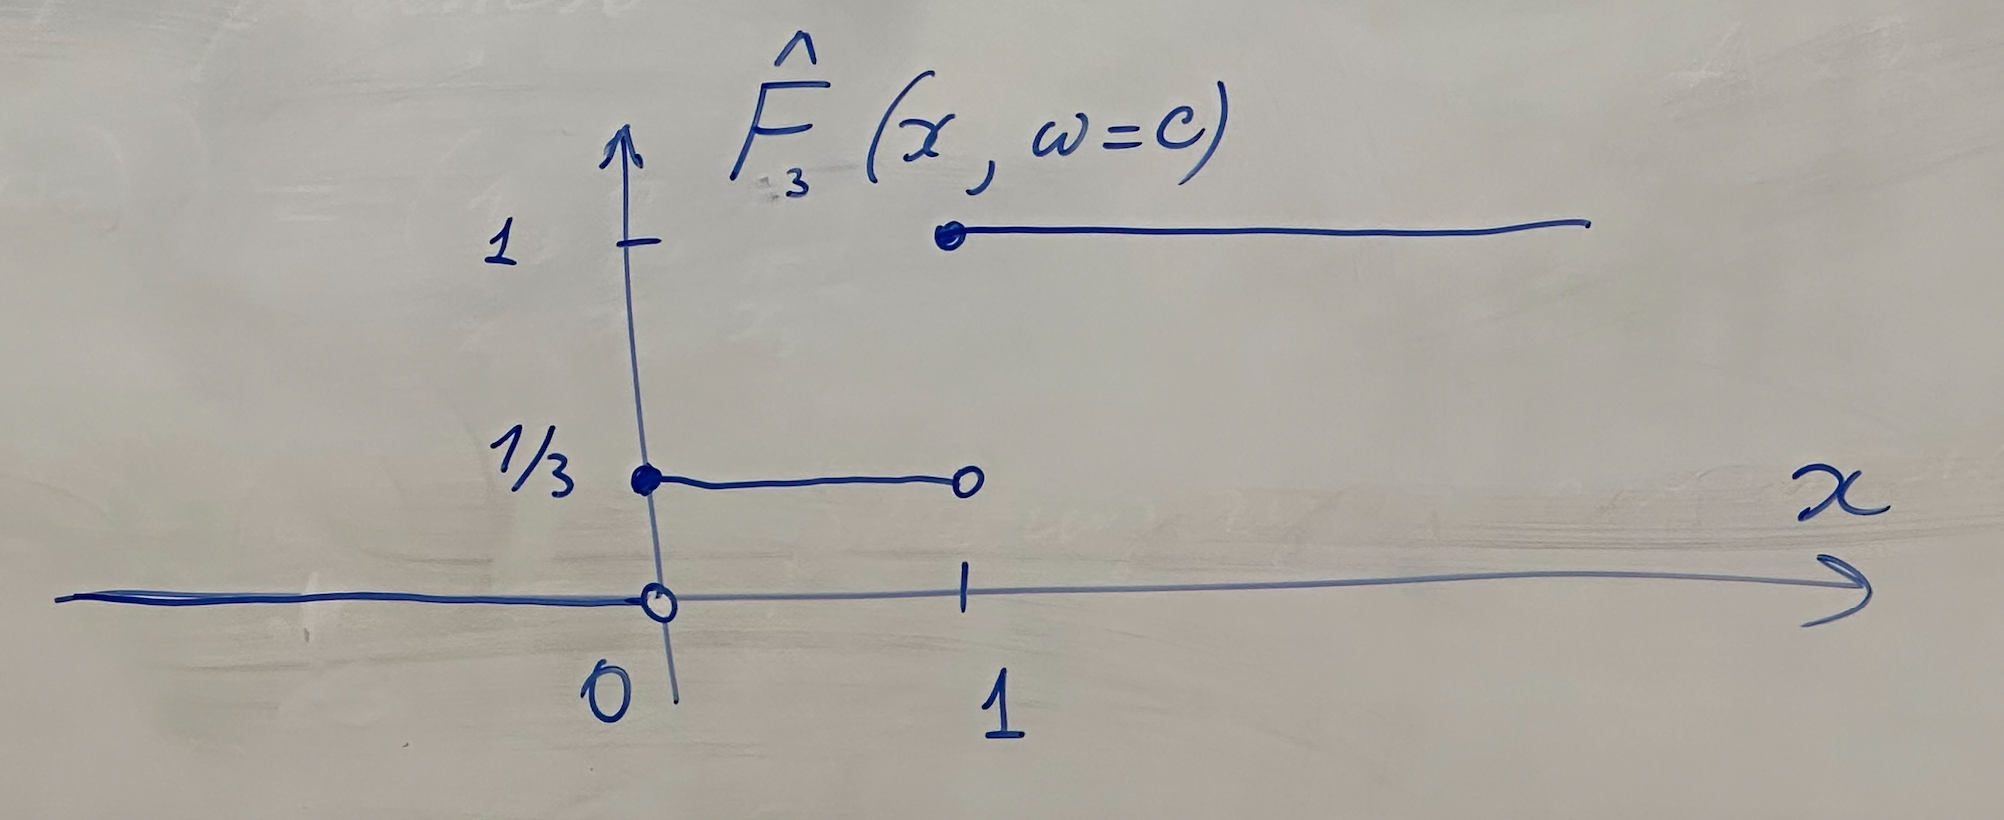
\includegraphics[width=0.6\linewidth]{intro-to-stat.png}
\end{figure}

\state Пусть $X=(X_1,\ldots,X_n)$ — случайная выборка, компоненты которой имеют конечное матожидание. Тогда 
\begin{equation*}
    \matwait{\overline{X}}=\matwait{X_i}
\end{equation*}

\state Пусть $X=(X_1,\ldots,X_n)$ — случайная выборка, компоненты которой имеют конечные дисперсии. Тогда 
\begin{equation*}
    \dispersia{\overline{X}}=\frac{\dispersia{X_i}}{n}
\end{equation*}

\proof \begin{equation*}
    \begin{aligned}
        \dispersia{\overline{X}}&=\dispersia{\frac{1}{n}\sum_{i=1}^nX_i}\\
        &=\frac{1}{n^2}\dispersia{\sum_{i=1}^nX_i}\\
        &=\frac{1}{n^2}\sum_{i=1}^n\dispersia{X_i}\\
        &=\frac{1}{n^2}n\dispersia{X_i}\\
        &=\frac{\dispersia{X_i}}{n}
    \end{aligned}
\end{equation*}

\definition Пусть $X=(X_1,\ldots,X_n)$ — случайная выборка из распределения с функцией распределения $F(x;\theta)$, где $\theta$ — неизвестный параметр

Оценкой параметра $\theta$ называется случайная величина $\hat{\theta}$, которая является произвольной борелевской функцией от элементов случайной выборки, то есть
\begin{equation*}
    \hat{\theta}=g(X_1,\ldots,X_n),
\end{equation*}
где $d:\mathbb{R}^2\longrightarrow\mathbb{R}$ — произвольная борелевская функция

\ex  $X=(X_1,\ldots,X_n)$ — случайная выборка из распределения Бернулли с параметром $p\in(0;1)$

$\hat{p}=\displaystyle\frac{X_1+\ldots+X_n}{n}$ — оценка параметра $p$

\definition Оценка $\hat{\theta}$ неизвестного параметра $\theta\in\Theta$ называется \textit{несмещенной}, если 
\begin{equation*}
    \matwait{\hat{\theta}}=\theta\ \forall\theta\in\Theta
\end{equation*}

\ex  $X=(X_1,\ldots,X_n)$ — случайная выборка из распределения Бернулли с параметром $p\in(0;1)$. Определим, является ли $\hat{p}=\frac{X_1+\ldots+X_n}{n}$ несмещенной оценкой для параметра $p$

\begin{equation*}
    \begin{aligned}
        \matwait{\hat{p}}&=\frac{\matwait{X_1+\ldots+X_n}}{n}\\
        &=\frac{\matwait{X_1}+\ldots+\matwait{X_n}}{n}\\
        &=\frac{np}{p}\\
        &=p
    \end{aligned}
\end{equation*}

То есть $\hat{p}$ — несмещенная оценка

\definition Говорят, что последовательность случайных величин $(X_n)_{n=1}^{\infty}$ сходится по вероятности к случайной величине $X$, если
\begin{equation*}
    \forall \varepsilon>0\ \lim\limits_{n\to\infty}\prob{|X_n-X|>\varepsilon}=0
\end{equation*}
Обозначение: $X_n\overset{\mathbb{P}}{\longrightarrow}X$ при $n\to\infty$ ИЛИ $p\lim\limits_{n\to\infty} X_n=x$

\definition Оценка $\hat{\theta}_n$ называется \textit{состоятельной оценкой} неизвестного параметра $\theta\in\Theta$, если
\begin{equation*}
    \forall \theta\in\Theta\ \hat{\theta}_n\overset{\mathbb{P}}{\longrightarrow}\theta\text{ при }n\to\infty
\end{equation*}

\ex Проверим, что $\hat{p}=\displaystyle\frac{X_1+\ldots+X_n}{n}$ является состоятельной. По ЗБЧ:
\begin{equation*}
    \begin{aligned}
        \hat{p}=\displaystyle\frac{X_1+\ldots+X_n}{n}\overset{\mathbb{P}}{\longrightarrow}\matwait{X_i}=p
    \end{aligned}
\end{equation*}
Значит, $\hat{p}$ — состоятельная оценка

\newpage
\section{Оптимальные оценки, характеристики выборок}
\subsection{Свойства оптимальных оценок}
% \definition $X_1,\ldots,X_n\sim F(x,\Theta)$
\definition Оценкой для параметра будет некоторая функция $\hat{\Theta}=T(X_1,\ldots,X_n)$

\definition Оценка \textit{состоятельна}, если $\hat{\Theta}\overset{\mathbb{P}}{\underset{n\to\infty}{\longrightarrow}}\Theta$

\definition Оценка \textit{желательно} должна обладать свойством \textit{несмещенности}, то есть $\matwait{\hat{\Theta}}=\Theta$

\ex $X_1,\ldots,X_n$. Построим две оценки
\begin{enumerate}
    \item $\hat{\mu_1}=\displaystyle\frac{1}{4}\left(X_1,\ldots,X_4\right)$ % — эта оценка лучше как минимум потому, что в ней веса каждого наблюдения равны
    \item $\hat{\mu_2}=\displaystyle\frac{1}{8}X_1+\frac{1}{8}X_2+\frac{1}{4}X_3+\frac{1}{2}X_4$
\end{enumerate}
Первая оценка лучше как минимум потому, что в ней веса каждого наблюдения равны

\definition Среднеквадратичная ошибка оценки — это 
\begin{equation*}
    \matwait{\hat{\Theta}-\Theta}^2
\end{equation*}

\begin{equation*}
    \begin{aligned}
        \matwait{\hat{\Theta}-\Theta}^2&=\matwait{\left(\hat{\Theta}-\matwait{\hat{\Theta}}\right)+\underbrace{\left(\matwait{\hat{\Theta}}-\Theta\right)}_{b(\Theta)\text{— смещение}}}^2\\
        &=\underbrace{\matwait{\hat{\Theta}-\matwait{\hat{\Theta}}}^2}_{\dispersia{\hat{\Theta}}}+b^2(\Theta)+2\underbrace{\matwait{\hat{\Theta}-\matwait{\hat{\Theta}}}}_{=0}\cdot b(\Theta)\\
        &=\underbrace{\matwait{\hat{\Theta}-\matwait{\hat{\Theta}}}^2}_{\dispersia{\hat{\Theta}}}+b^2(\Theta)
    \end{aligned}
\end{equation*}

\definition $\hat{\Theta}_1$ эффективнее, чем $\hat{\Theta}_2$, если
\begin{equation*}
    \begin{aligned}
        \matwait{\hat{\Theta_1}-\Theta}^2&\leqslant\matwait{\hat{\Theta_2}-\Theta}^2\text{причем }\exists \Theta_0:\\
        \matwait{\hat{\Theta_1}-\Theta_0}^2&<\matwait{\hat{\Theta_2}-\Theta_0}^2
    \end{aligned}
\end{equation*}


\definition Оценка $\hat{\Theta}$ называется эффективной (=оптимальной, $the\ best$) в классе $K$, если $\forall\ \overline{\Theta}\in K$
\begin{equation*}
    \begin{aligned}
        \matwait{\hat{\Theta}-\Theta}^2&\leqslant\matwait{\overline{\Theta}-\Theta}^2\text{причем }\exists \Theta_0:\\
        \matwait{\hat{\Theta}-\Theta_0}^2&<\matwait{\overline{\Theta}-\Theta_0}^2
    \end{aligned}
\end{equation*}
Класс $K$ обладает смещением $b(\Theta)$

\definition Оценка $\hat{\Theta}$ называется эффективной в классе несмещенных оценок, если $\forall\ \overline{\Theta}\in K$
\begin{equation*}
    \begin{aligned}
        \dispersia{\hat{\Theta}}&\leqslant \dispersia{\overline{\Theta}},\text{причем }\exists \Theta_0:\\
        \dispersia{\hat{\Theta}}&< \dispersia{\overline{\Theta}}\text{для }\Theta_0
    \end{aligned}
\end{equation*}

\subsection{Способы организации выборки}
\definition Генеральная совокупность — выборка, которая в теории может быть доступна, но на практике вряд ли ее можно собрать. Например, точное население РФ

\begin{enumerate}
    \item Простой случайный отбор — практически нереализуемо
    \item Отбор с помощью механистической процедуры, не влияющий на случайность
    
    Например, на автоматическом производстве надо посчитать процентр брака. Тогда, для выборки можно ограничиться промежутком времени 14:20-14:30

    \item Стратифицированные выборки — выборка производится из страт, то есть берут людей из всех социальных слоев населения
    \item Комбинирование 
\end{enumerate}
Таким образом, важно следить, чтобы выборка обладали всеми или большинством свойств генеральной совокупности

\subsection{Характеристики выборки}
\begin{enumerate}
    \item Вариационный ряд — наблюдения, упорядоченные по возрастанию
    \begin{equation*}
        X_{(1)}\leqslant X_{(2)}\leqslant\ldots\leqslant X_{(n)}\text{— случайные величины}
    \end{equation*}
    При этом, $X_{(1)}$ и $X_{(n)}$ — экстремальные статистики

    \item Гистограмма и выборочная функция распределения
    
    \definition Выборочная (эмпирическая) функция распределения — это $$\hat{F}_n(x)=\displaystyle\frac{\sum_{i=1}^{n}I\{X_i\leqslant x\}}{n},$$ где $I\{X_i\leqslant x\}$ — индикаторная функция, показывающая сколько наблюдений меньше либо равны какого-то $x$

    \definition $\hat{p}_i=\displaystyle\frac{m(\delta i)}{|\delta i|\cdot n}$, где $m(\delta i)$ — число наблюдений, попавших в интервал $\delta i$, $|\delta i|$ — длина интервала, $n$ — число наблюдений

    Гистограмма — тоде своего рода функция плотности
\end{enumerate}











\end{document}